\documentclass[a4,center,fleqn]{NAR}
\usepackage{hyperref}
\usepackage{graphicx}
\usepackage{csquotes}
\usepackage{amsmath}
\usepackage{setspace}
\usepackage{float}
\usepackage{caption}

\begin{document}
\section{Abstract}

In this study, we plan to find dissimilarities between normal cells and cancerous cells,
through investigating HiC contact maps. 
We suspect that there are systematic differences between how chromosomes are structured
between normal cells and cancerous cells.
we 
Ideally, it is desirable to compare 3D structures of 
cell in order to make such comparisons.
However, the main challenge that we face is that 
3D structure of a cell is not readily available. Based on
\cite{adhikari2016chromosome3d}, fluorescence in situ hybridizaiton
(FISH) is used for investigating 3D configuration of chromosomes.
However, this method can only be used locally and cannot map
the whole structure of the chromosomes.
In orther to find dissimilarities in the 3D structure of 
chromosomes, we used HiC dataset.
The HiC method, which was developed by \cite{lieberman2009comprehensive}, captures interactions between 
chromosomal fragments in kilobase resolution. Based on HiC data, an
\textit{interaction frequency (IF) } matrix can be developed between \textit{loci} at a desired resolution.
A cell $IF_{ij}$ in an interaction frequency matrix captures the number of interaction detected
in HiC dataset between locus $i$ and locus $j$ in the genome.
An interaction matrix can be used to develop both inter- and intra-chromosomal interaction matrices.
We believe differences in interaction matrices can be found between normal cells and cancerous ones.

\section{Introduction}

Graphlet comparison is a novel method used to compare large networks in order to
find local similarities in them.
Authors of \cite{prvzulj2007biological} provide a new measure of PPI
network comparison
based on 73 constraints. This is used in order to compare two large
networks in order to detect similarities.

\cite{milenkoviae2008uncovering} 
 provide heuristics to compare two nodes based on some feature
(or signature) vectors, which is a 73-dimensional vector
$\mathbf{s}^T
= [s_0, s_2, ..., s_{72}]$ where $s_i$ denotes the number of nodes in
the network that are part of an orbit $i$. \\
\textit{Important Result}: Proteins with similar surroundings perform
similar functions.

In \cite{milenkovic2010cancer}, the same author investigates 
cancer-causing genes to find similarities in their signatures. After
clustering the genes based on \textit{signature similarity} criteria,
some clusters contain a lot of cancerous genes.
They use 4 different clustering methods with varying parameters to cluster
the proteins. They then predict the cancer-relatedness of a protein 
$i$ using
an enrichment criteria $\frac{k}{|C_i|}$ where $C_i$ is the cluster
where protein $i$ belongs and $k$ is the number of cancer-causing
proteins in $C_i$ and $|C_i|$ is the size of $C_i$.


The authors of \cite{di2010fast} generalized the idea of graphlets to 
ordered graphs were the nodes are labeled in ascending order.
As can be viewed, there are a total of 14 orbits for graphlets of size
2 and 3 since the label of graphlets is also included in toplogy.
In the new definition, $d_v^i$ denotes the number of orbit $i$ touches 
node $v$. Each node, is then assigned a vector of length 14 
\footnote{number of orbits in graphlets of size 2 and 3}
$(d_v^1, d_v^2, ..., d_v^{14})$ 
and similarity of two nodes in two contact maps can be compared by
how geometrically close their corresponding vectors are.
\section{Materials and Methods}
\subsection{Thresholding contact maps}
In order to be able to extract graphlets, HiC contact maps should be modeled as
unweighted graphs where the nodes represent the loci and an edge between two 
nodes represent a \textit{significant} interaction between the loci the nodes
represent.

Thresholding is achieved by thresholding the contact maps. The result
of the thresholding procedure would be a binary matrix which also can serve as
an adjacency matrix for an unweighted, undirected graph. The graph can then be
used for orbit extraction.

In order to go about the process of thresholding, it is necessary to make sure
that both global and local features are maintained. We could consider 
thresholding the contact maps by simply setting values above a fixed value to
one and the rest to zero. However, in practice, this proved result in graphs
that capture the local structure of the contact maps poorly. This is because
intensities follow an exponential distribution with a mean close to zero and
some very larges values that correspond t interactions along and close to 
the main diagonal of the contact maps.
Thus, picking relatively large numbers would result in ignoring interactions
that are far from the main diagonal and picking small numbers will lead to
capturing too many \textit{insignificant} interactions.

In order to threshold the matrix so that both global and local patterns are
kept, we borrowed the concept of \textit{adaptive thresholding} from image 
processing context. In this method, in order to be set, a pixel should have
an intensity that is larger than the average of non-zero intensities in its
\textit{neighborhood}. The neighborhood is defined by an sliding kernel 
that passes through the contact map with a pixel at its middle at 
each step. Figure \ref{local_thresholded_chr1_chr1} demonstrates result of 
this thresholding approach for interchromosomal contact map of chromosome 1.
Refer to supplementary material for all 23 interchromosomal thresholding
results.
\begin{figure*}[t]
    \centering
    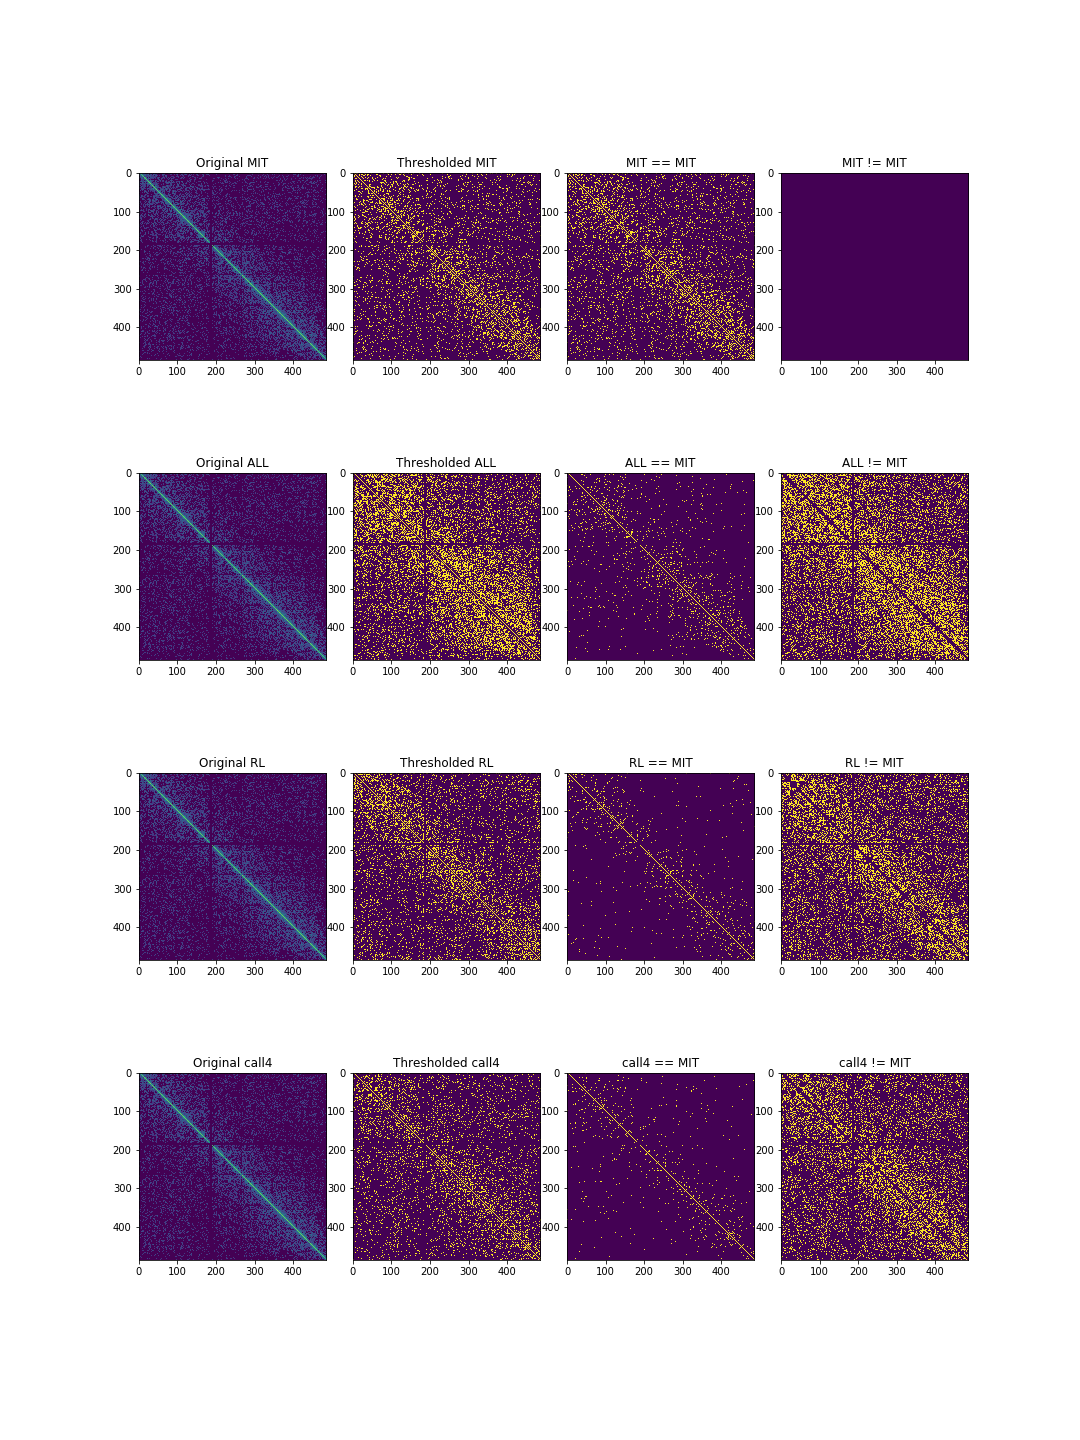
\includegraphics[width=\textwidth]{figures/local_thresholded_chr1_chr1.png}
    \caption{Result of thresholding interchromosomal contact map of chromosome 1
    using a kernels of size $5 \times 5$. The first row shows the thresholded
    maps. Second and third rows demonstrate pair-wisesimilarities and 
    differences between contact maps respectively.}
    \label{local_thresholded_chr1_chr1}
\end{figure*}

\subsection{Orbit Extraction}
Once the thresholded contact maps are obtained, graphlets and orbits can be 
extracted. We used the \texttt{orca} package in \texttt{R} programming 
language to extract the graphlets. As a result of graphlet extraction, 
For each loci in each contact map, a \textit{signature vector} of size
73 is created.

We divied the task of graphlet comparison into two parts: first we compare
graphlets from each contact map in normal cell lines (MIT) with the 
same contact maps in the other three Leukemic cells. Second we compare 
contact maps in a similar way but this time only between leukemic cells.
In the former case, the null hypothesis is that there is no difference
between contact maps of normal cells and leukemic celss and in the later
case, the null hypotheis is that there is no difference between 
different leukemic cells.

We consider two measures of \textit{difference} when comparing contact
map graphlets. The first measure is the distance between signature vectors
of a loci in two cell lines. If $S^A_{k}$  and $S^B_{k}$ are 
signature vectors corresponding to loci $k$ in contact maps A and B 
respectively, then we can caclulate the distance between the two loci 
using the following formula from \cite{prvzulj2007biological}:

\begin{equation}
    d_{ki} = w_i \times \frac{log(S^A_{ki}+1) - log(S^B_{ki}+1)}{log(max(S^A_{ki}, S^B_{ki}) + 2)}
\end{equation}
The distance between $S$ and $S'$ can be calculated as follows:
\begin{equation}
    D(S^A_k, S^B_k) = \sqrt{\sum_{0}^{72}{d_{ki}^2}}
\end{equation}


Using this distance measure, we can quantify how two loci are close to
each other in terms of local neighborhood between the two contact maps.

The second measure of comparison that we use captures how 
similar two orbits are in terms of their frequencies across loci
between the two contact maps. For each contact map, we can calculate
similarity between orbit distributions by calculating pearso's r 
correlation. However, pearson's r might not be able to capture
non-functional relationships between distributions. As a result, we
also used Maximal Information Coefficient (MIC) 
\cite{reshef2011detecting} in order to compare
correlations. MIC calculates mutual information (MI) between two
distributions, but utilizes dynamic programming in order adjust
bin sizes and numbers in order to achieve highest MI.
MIC values between two variables fall between 0 and 1,
with 0 meaning that the two variables are completely independent
and 1 meaning they are totally correlated.
We used both Pearson's r and MI in order to compare orbit
frequencies. Although results from both approaches were more
or less consistent, MIC showed higher robustness than Pearson's 
r method.

\subsection{Hypotheses}
\subsubsection{terminology}
We denote the set of all contact maps of normal (MIT) cell line with
$CM$. In the same manner we denote $CA$, $CR$ and $CC$ as the set of all
contact maps corresponding to ALL, RL and CALL4 cell lines.
We denote a member of any of the aforementioned sets using small
letters of the set name. For example, we denote any member of $CA$ with
$ca$.

We denote a contact map by $C^{\{cell_{\{chr1\}\{chr2\}}\}}$, where the
superscript denotes the cell type and the subscripts in the superscripts
determines the pair of chromosomes the contact map is about. For 
example $C^{MIT_{1,14}}$ denotes the contact map between chromosomes
1 and 14 in MIT (Normal) dataset. In such a manner $C^{MIT_{1,14}}_{ij}$
denotes the interaction between loci $i$ and $j$ in the aforementioned
contact map.

We denote $S^C_i$ as the extracted 
signature vector of locus $i$ in contact map $C$. 
Also $P^C_k$ denotes
the frequency distribution of orbital $k$ in contact map $C$.

With regard to the two aforementioned comparison methods, we define
our two null hypotheses as the following:

\begin{enumerate}
    \item For a locus in a contact map in MIT cell type, its distance
        from the same locus in the same contact map of the other three
        cell types are equal to $0$.
            \begin{align}
                \begin{split}
                    H_0: D(sm, sa) = 0  \\
                \hspace{.5cm} \forall cm \in CM \quad\&\quad ca \in CA
                \end{split} \\
                \begin{split}
                    H_0: D(sm, sr) = 0   \\
                \hspace{.5cm} \forall cm \in CM\quad \&\quad cr \in CR
                \end{split} \\
                \begin{split}
                    H_0: D(sm, sc) = 0   \\
                \hspace{.5cm} \forall cm \in CM\quad \&\quad cc \in CC
                \end{split}
            \end{align}
    \item For an orbit extracted from a contact map of MIT cell, the 
        Pearson's r correlation between its frequency and the frequency
        of the same orbit extracted from the same contact map in 
        the other three cell types in equal to 1.
        \begin{align}
            H_0: Corr(P^CM_k, P^CA_k) = 1 \\
            H_0: Corr(P^CM_k, P^CR_k) = 1 \\
            H_0: Corr(P^CM_k, P^CC_k) = 1
        \end{align}

        or

        For an orbit extracted from a contact map of MIT cell, the 
        MIC between its frequency and the frequency
        of the same orbit extracted from the same contact map in 
        the other three cell types in equal to 1.
\end{enumerate}



\newpage
\section{Resources}
\textbf{Hi-C Datasets:}
\begin{enumerate}
    \item \href{https://github.com/rasoolianbehnam/watson}{Code base for this article}
    \item \href{http://sysbio.rnet.missouri.edu/T0510/tmp_download/link_to_download_genome_data/}
        {Datasets including cancerous cells}
    \item \href{https://bcm.app.box.com/v/aidenlab/folder/11234760671}{Original Datasets}
\end{enumerate}


\bibliography{lit}
\bibliographystyle{unsrt}
\end{document}
